\documentclass[11pt]{article}
\usepackage[T1]{fontenc}
\usepackage[english]{babel}
\usepackage{csquotes}
\usepackage[margin=1in]{geometry}
\usepackage{amsmath}
\usepackage{graphicx}
\usepackage{booktabs}
\usepackage{siunitx}
\usepackage[style=numeric]{biblatex}
\addbibresource{references.bib}
\usepackage[colorlinks=true, allcolors=blue]{hyperref}

\begin{document}

\pagenumbering{alph}
\begin{titlepage}
  \centering
  {\large Institution \par}
  {\large Department \par}
  \vspace{4cm}
  {\scshape Lab report \par}
  \vspace{1cm}
  {\huge\bfseries {{TITLE}} \par}
  \vspace{2cm}
  {\Large {{AUTHOR}} \par}
  \vspace{1cm}
  Submitted to Professor's name \par
  Course CODE1234 \par
  \vfill
  {\large \today \par}
\end{titlepage}
\pagenumbering{arabic}

\tableofcontents
\newpage

\section{Objectives}

This section states in a few lines the aim of the experiment or project and
the question it answers.

\section{Materials and methods}

\subsection{Materials}

\begin{itemize}
  \item a digital oscilloscope,
  \item a function generator,
  \item an RC circuit with a \qty{10}{\kilo\ohm} resistor and a
        \qty{100}{\nano\farad} capacitor.
\end{itemize}

\subsection{Method}

A step voltage is applied to the circuit and the voltage across the
capacitor is measured. The time constant of the circuit is
\begin{equation}
  \tau = RC = \qty{1}{\milli\second}.
  \label{eq:tau}
\end{equation}

\section{Results}

Table~\ref{tab:measurements} lists the measurements and
Figure~\ref{fig:results} plots them.

\begin{table}[htbp]
  \centering
  \caption{Voltage across the capacitor.}
  \label{tab:measurements}
  \begin{tabular}{S[table-format=1.1] S[table-format=1.2]}
    \toprule
    {Time (\unit{\milli\second})} & {Voltage (\unit{\volt})} \\
    \midrule
    0.0 & 0.00 \\
    0.5 & 1.97 \\
    1.0 & 3.16 \\
    2.0 & 4.32 \\
    5.0 & 4.97 \\
    \bottomrule
  \end{tabular}
\end{table}

\begin{figure}[htbp]
  \centering
  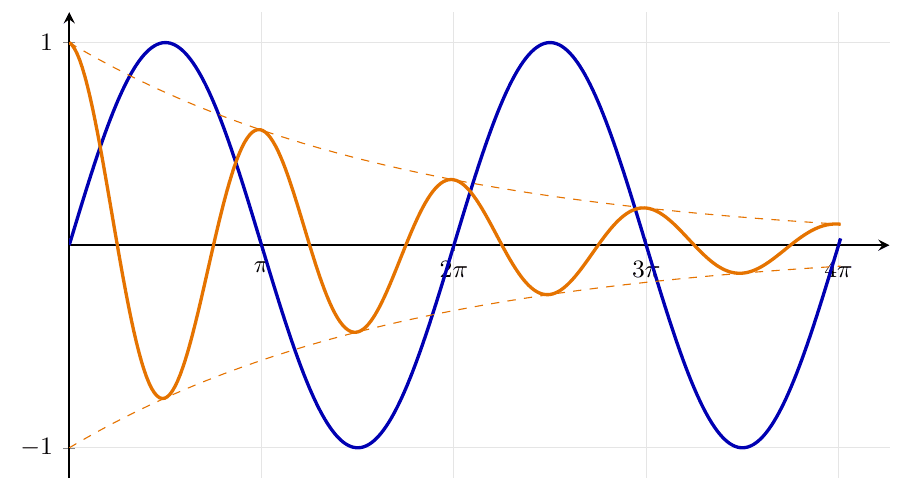
\includegraphics[width=0.75\linewidth]{images/curves.png}
  \caption{An image of the project: replace it with your results.}
  \label{fig:results}
\end{figure}

\section{Discussion}

The results are compared with the theory of Equation~\eqref{eq:tau} and the
differences observed are explained \parencite{taylor1997}.

\section{Conclusion}

The conclusion answers the question asked in the objectives.

\printbibliography[heading=bibintoc]

\appendix
\section{Raw data}

The appendices hold what would weigh down the report: raw data, detailed
calculations, code.

\end{document}
